\documentclass[sfheadings,a4paper,times,9pt,floats,floatfix]{article}
\usepackage[margin=0.7in]{geometry}
\usepackage{graphicx}
\usepackage{verbatim}
\usepackage{bookmark}
\usepackage{url}% to fix the figure at the exact position
% \restylefloat{figure}
%\usepackage{hyperref}
\usepackage{mathrsfs}
\usepackage{amssymb}
\usepackage{amsmath}
\usepackage{bm}
\usepackage{color}
\usepackage[table]{xcolor}% http://ctan.org/pkg/xcolor
\usepackage{multirow}
\usepackage{caption}
\usepackage{subfig}
\usepackage{afterpage}
\usepackage{floatrow}
\floatsetup[table]{capposition=top}

% \voffset .5in
\title{SKA1-Mid Scale-Dependent Sensitivity}
\author{O. M. Smirnov$^{1,2}$, S. Makhathini$^{1,2}$, M. Jarvis$^{3,4}$, F. B. Abdalla$^5$ \\{\footnotesize \it $^1$Rhodes
University, South Africa $^2$SKA South Africa, $^3$ University of the Western Cape, South Africa,}\\ {\footnotesize \it
$^4$University of Oxford, $^5$Department of Physics and Astronomy, University College London}}
\date{}
\begin{document}
\maketitle
\vspace{-1.1cm}
\begin{abstract}
 In this report we study the scale dependent sensitivity of the SKA1-Mid baseline design. We also propose changes to the baseline
design that enhance the sensitivity at smaller angular scales (say 0.4-1 arcsec at 650MHz) without compromising the performance at
larger scales. The changes we propose are guided by the SKA1-Mid level-zero science requirements \cite{srd}, which suggest that
baselines larger than 100km are not necessary to achieve the SKA1-Mid science objectives. The layouts we propose could be
transformational for other potential science cases which are possible with such an instrument, such as cosmology with weak
lensing, at no significant cost to any of the key science cases. Furthermore, some of these layouts span significantly less space
which could potentially reduce trenching and data transport costs.
\end{abstract}

\section{Introduction}
\vspace{-.1cm}
The Square Kilometre Array (SKA) project is meant to be an international facility that will provide as much science as possible
during its lifetime. Although there is a large emphasis on key science projects outlined in several SKA memos, as the baseline
design \cite{bd} has emerged, it shall however be noted that changes which do not compromise the key science missions are possible
and such changes could be transformational for other potential science missions. In this short report, we compare the
scale-dependent sensitivity of the SKA1-Mid baseline design to 4 alternative designs. The alternative layouts we propose are
guided by the SKA1-Mid general science requirements outlined in the SKA1 Level-zero requirements document \cite{srd}, and the
possibility of having better imaging quality with SKA-Mid. Essentially, looking that at the SKA1-Mid science requirements
\cite{srd}, it is clear that baselines longer than about 100km are not a necessity. We therefore seek a layout with the shortest
possible maximum baseline that does at least as well as the ``second generation'' baseline design in the resolution range 0.4-1
arcsec over 650, 800 and 1100MHz\footnote{This well covers the highest resolution requirements in the level-zero science
requirements} while not significantly compromising the performance at the larger angular scales. Moreover, having a layout which
performs just as well as (or better) than the baseline layout but which covers significantly less space translates to less
trenching, which may present the opportunity to re-invest the funds somewhere else, therefore we consider the conservative
addition of 12 dishes. However, we note that improvements on the scales of interest are still possible without these 12 additional
dishes. In the next section we present 4 alternative layouts, these layouts have maximum baselines of 90,100,120 and 133 km. The
scale dependent sensitivity of these layouts is compared to the baseline layout in section \ref{sec:exp}, and our conclusions are
in section \ref{sec:conclusion}.

\subsection{Background on Layouts}\label{sec:layouts}
\vspace{-.1cm}
The following SKA1-Mid layouts are under consideration here:
\begin{description}
\item[{\bf REF2A100B173 :}] This is the ”Second-generation” layout (254 dishes) produced by Robert Braun (September
2013)\footnote{We assume this to be the baseline layout.}. The spiral arms of this layout stretch out to ~100km, and the maximum
baseline is 173km. In this report, we also refer to this layout as REF2. \item[{\bf X$i$-$j$A$k$B$l$ :}] This is the REF2 layout
with the core (within a 300m radial distance from the the centre) ``puffed up'' by 10\%, $i$ dishes moved from the outer core
(between a radial distance of 0.3 and 4km from the center) to the spiral arms and $j$ extra dishes added to the spiral arms. The
spacing in the arms is then optimized to get more sensitivity on the longer ($>50$km) baselines (See baseline distribution
histograms in Figure \ref{fig:hist} ). Each spiral arm stretches out to ~$k$ kilometres and the maximum baseline length is about
$l$ kilometres.
\end{description}
The  layouts are shown in Figure \ref{fig:lay}, and Figure \ref{fig:hist} shows the baseline distribution histogram for the
different layouts. Figure \ref{fig:uvcov} shows the uv-coverage for the different layouts at 1.1GHz at declination -30 degrees for
8hr tracks. At this point some optimisations have been done on the antenna distributions but we emphasise that further
improvements can be and should be made.
\begin{figure}[!htb]
\vspace{-.5cm}
 \tiny{%%% autogen
 \begin{tabular}{cccccc}
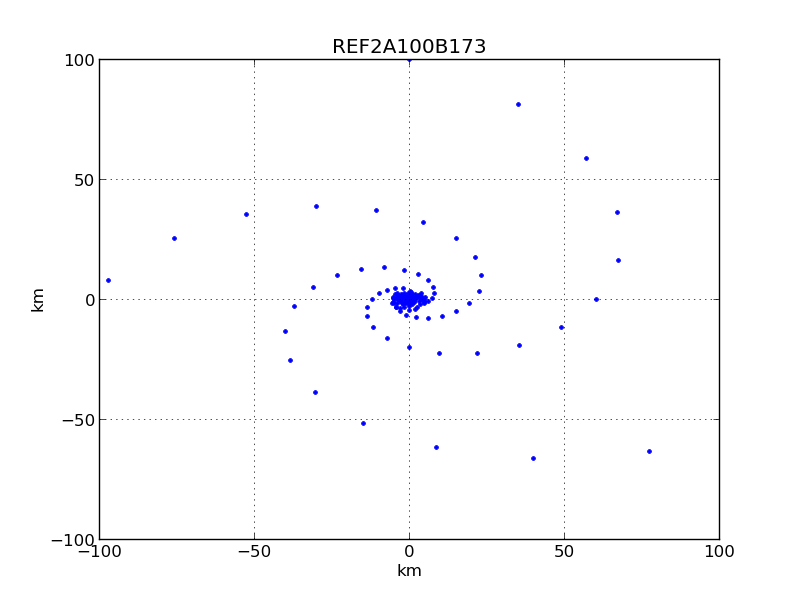
\includegraphics[width=0.150000\textwidth,trim= 0 .05cm 0 0.05cm]{{images/lay_SKA1REF2}.png} &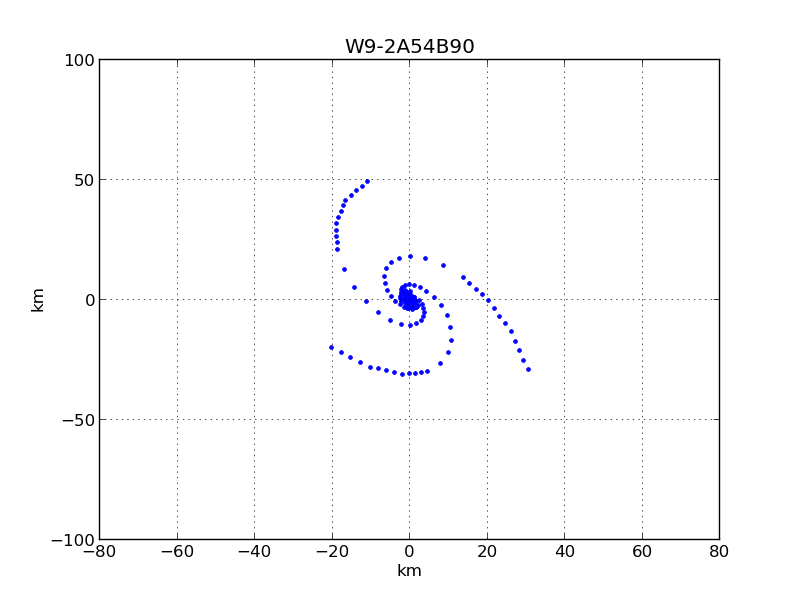
\includegraphics[width=0.150000\textwidth,trim= 0 .05cm 0 0.05cm]{{images/lay_SKA1W9-12A54B90}.png} &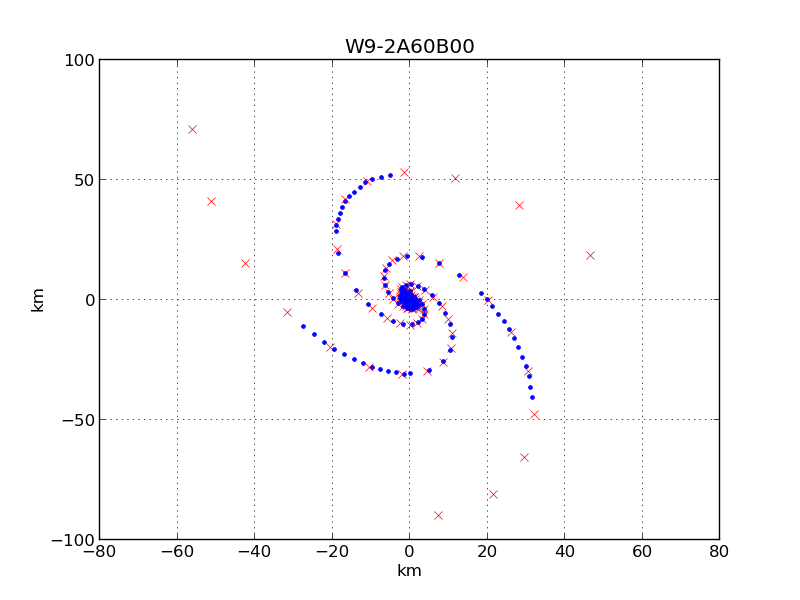
\includegraphics[width=0.150000\textwidth,trim= 0 .05cm 0 0.05cm]{{images/lay_SKA1W9-12A60B100}.png} &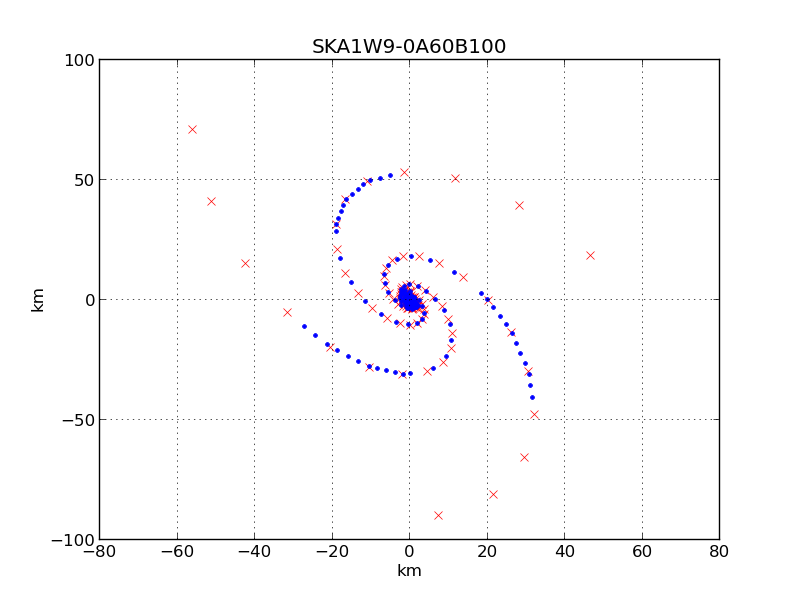
\includegraphics[width=0.150000\textwidth,trim= 0 .05cm 0 0.05cm]{{images/lay_SKA1W9-0A60B100}.png} &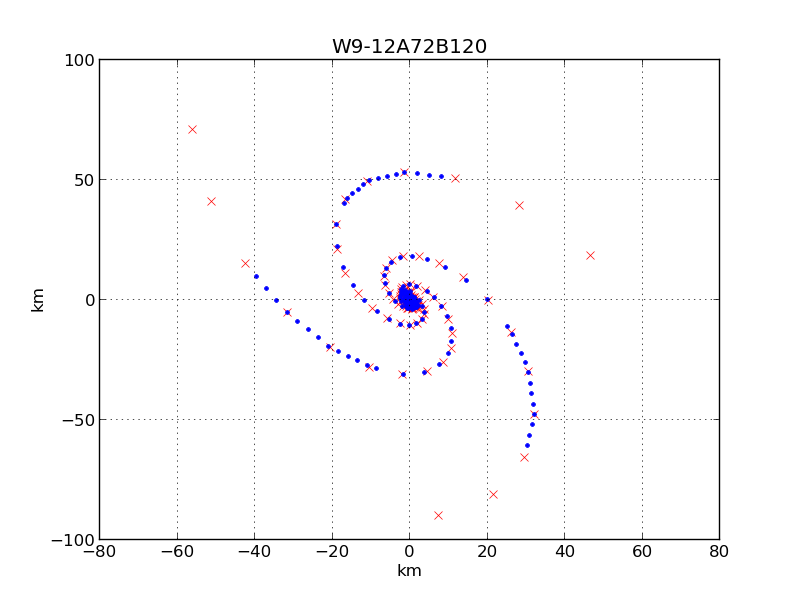
\includegraphics[width=0.150000\textwidth,trim= 0 .05cm 0 0.05cm]{{images/lay_SKA1W9-12A72B120}.png} &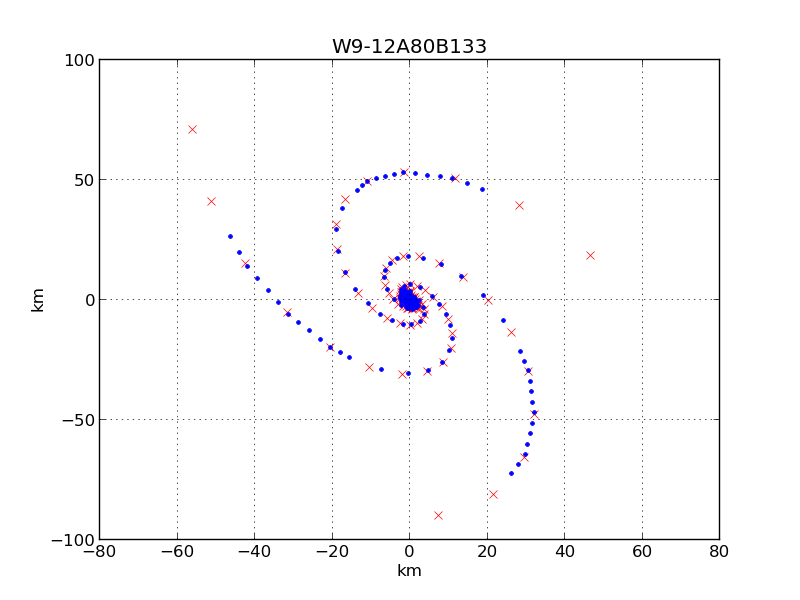
\includegraphics[width=0.150000\textwidth,trim= 0 .05cm 0 0.05cm]{{images/lay_SKA1W9-12A80B133}.png} 
 \\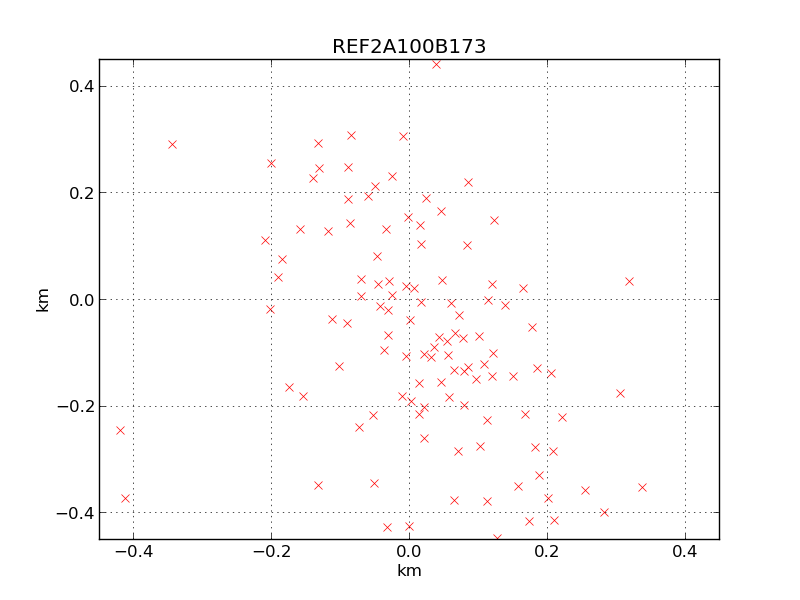
\includegraphics[width=0.150000\textwidth,trim= 0 .05cm 0 0.05cm]{{images/core_SKA1REF2}.png} &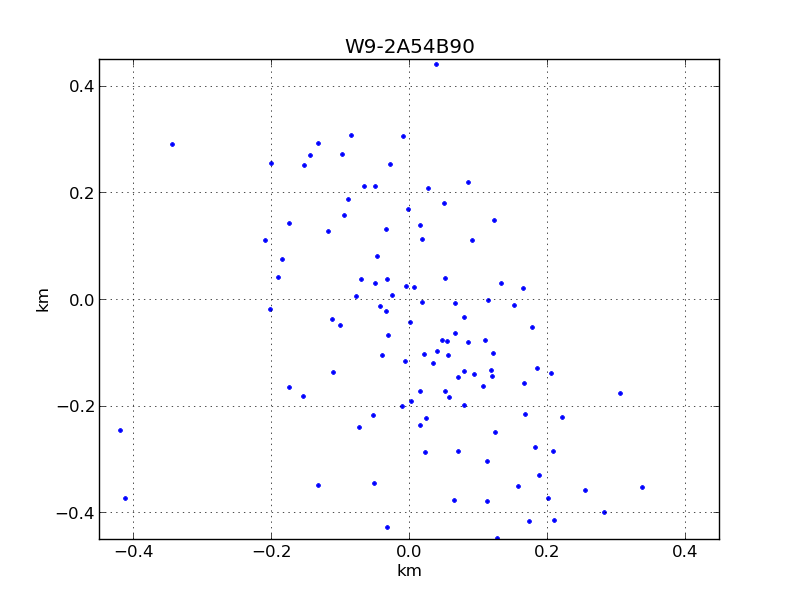
\includegraphics[width=0.150000\textwidth,trim= 0 .05cm 0 0.05cm]{{images/core_SKA1W9-12A54B90}.png} &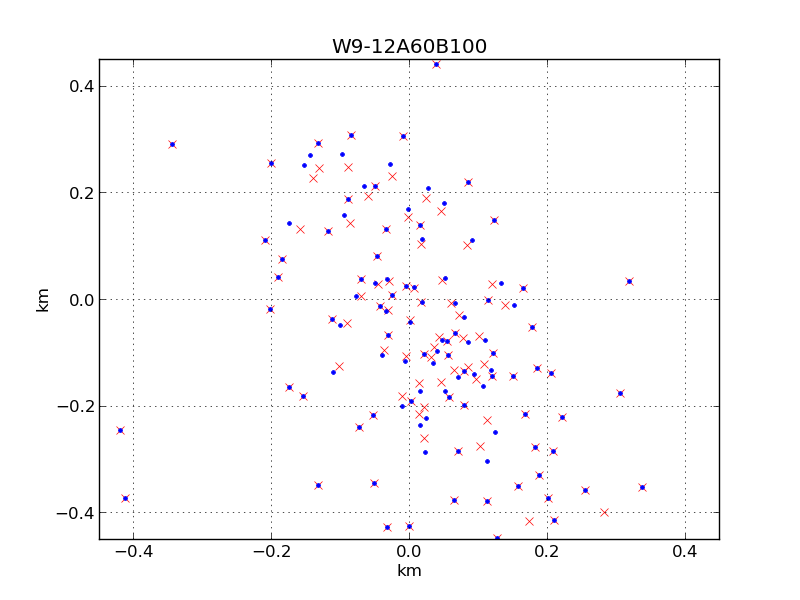
\includegraphics[width=0.150000\textwidth,trim= 0 .05cm 0 0.05cm]{{images/core_SKA1W9-12A60B100}.png} &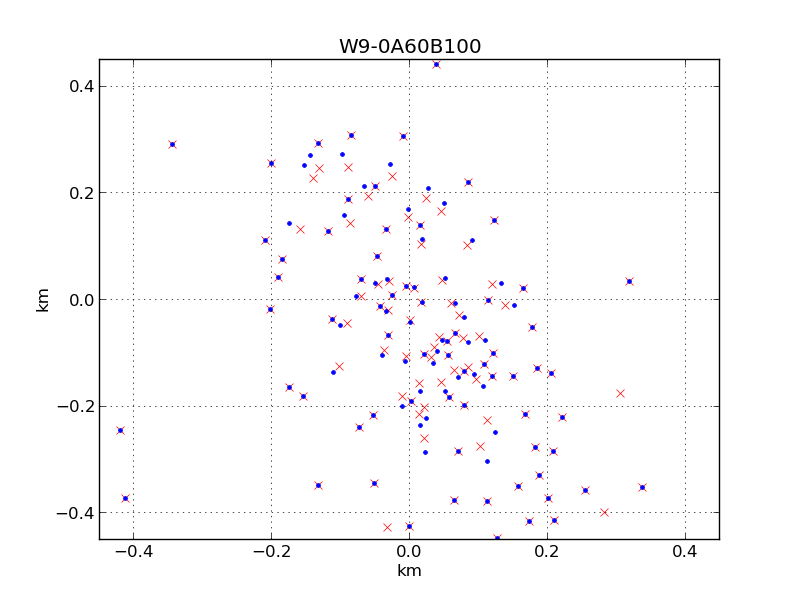
\includegraphics[width=0.150000\textwidth,trim= 0 .05cm 0 0.05cm]{{images/core_SKA1W9-0A60B100}.png} &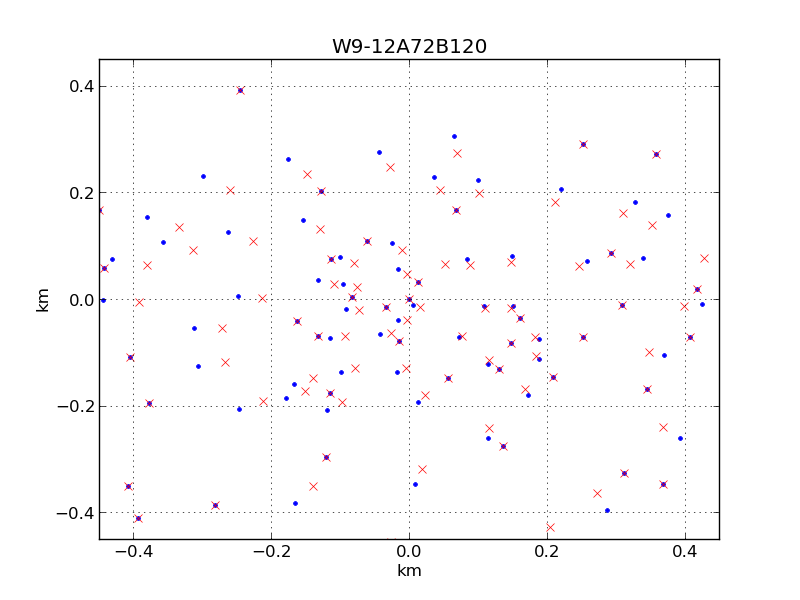
\includegraphics[width=0.150000\textwidth,trim= 0 .05cm 0 0.05cm]{{images/core_SKA1W9-12A72B120}.png} &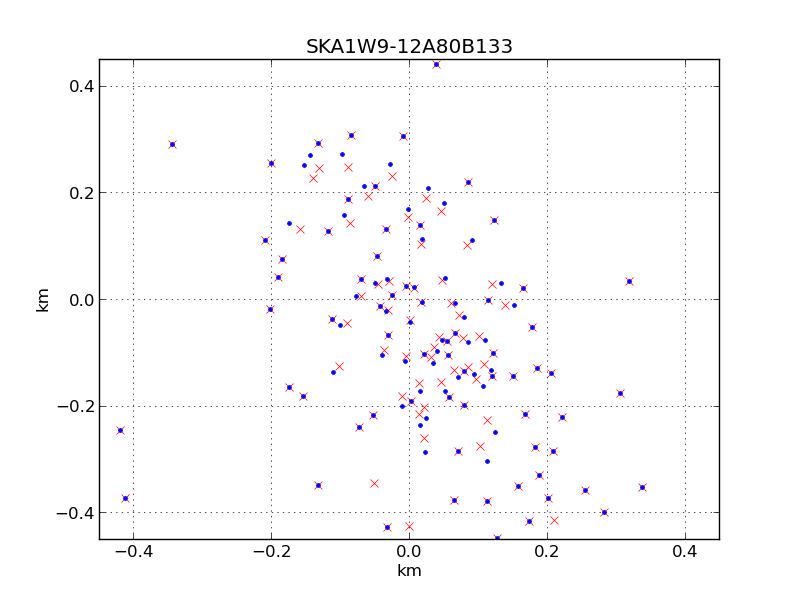
\includegraphics[width=0.150000\textwidth,trim= 0 .05cm 0 0.05cm]{{images/core_SKA1W9-12A80B133}.png} 
 \\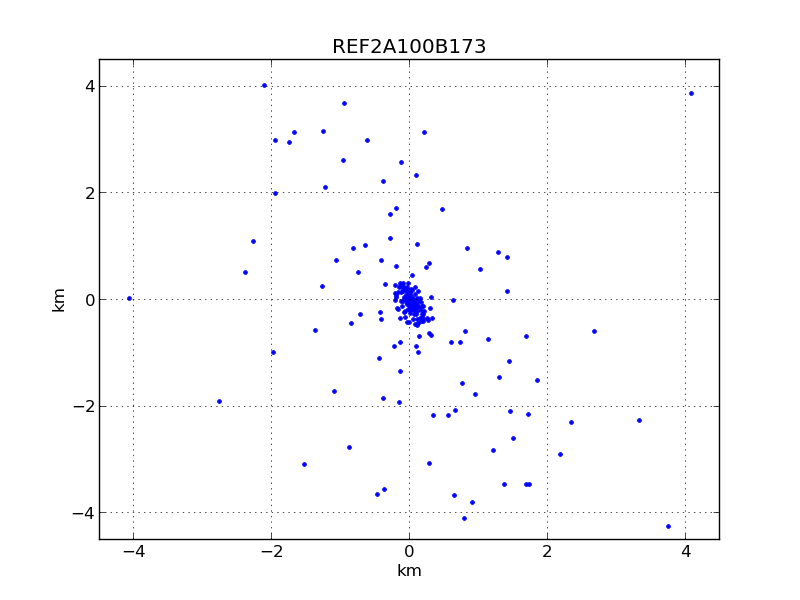
\includegraphics[width=0.150000\textwidth,trim= 0 .05cm 0 0.05cm]{{images/outer_core_SKA1REF2}.png} &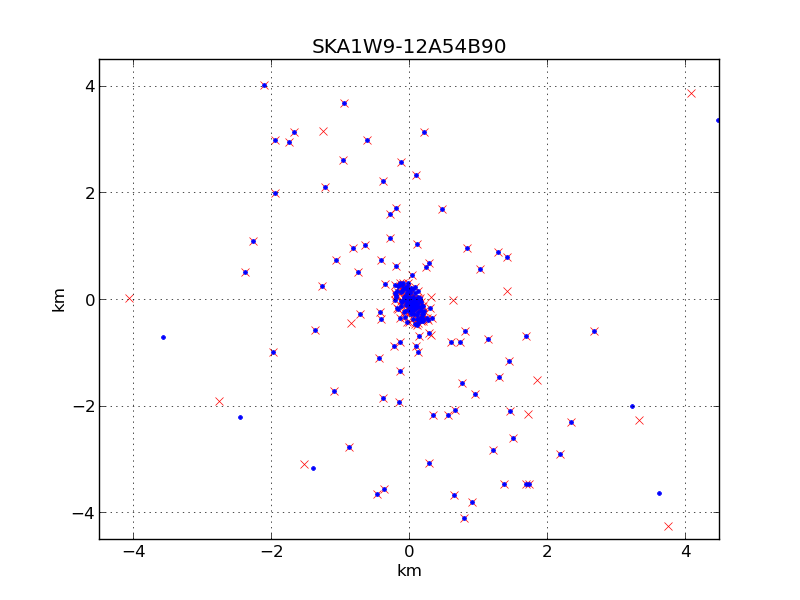
\includegraphics[width=0.150000\textwidth,trim= 0 .05cm 0 0.05cm]{{images/outer_core_SKA1W9-12A54B90}.png} &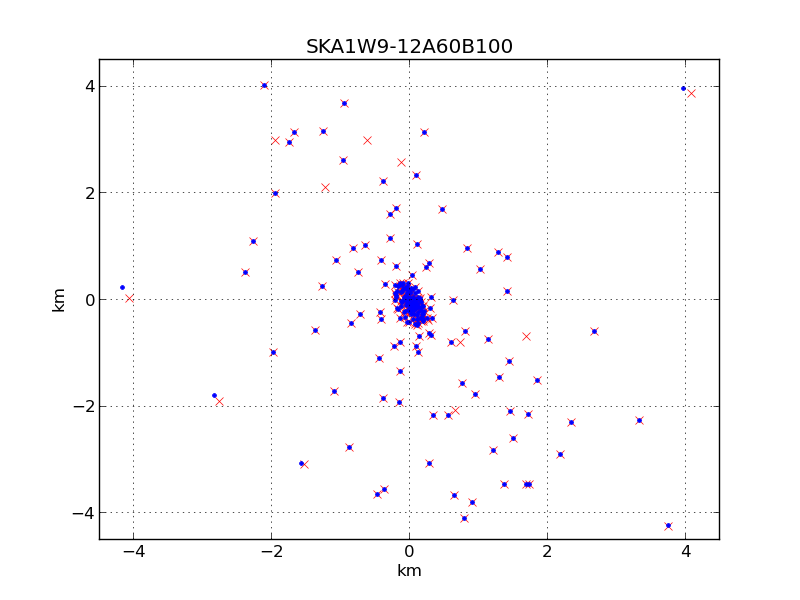
\includegraphics[width=0.150000\textwidth,trim= 0 .05cm 0 0.05cm]{{images/outer_core_SKA1W9-12A60B100}.png} &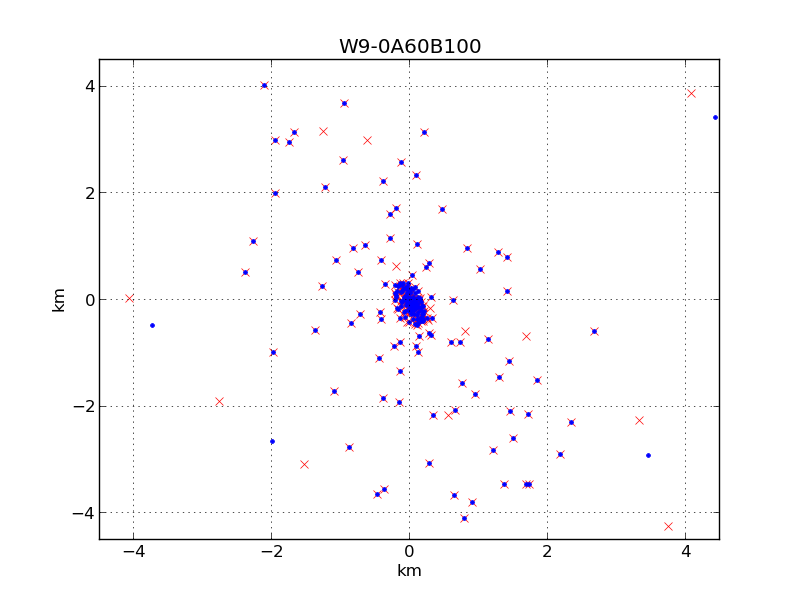
\includegraphics[width=0.150000\textwidth,trim= 0 .05cm 0 0.05cm]{{images/outer_core_SKA1W9-0A60B100}.png} &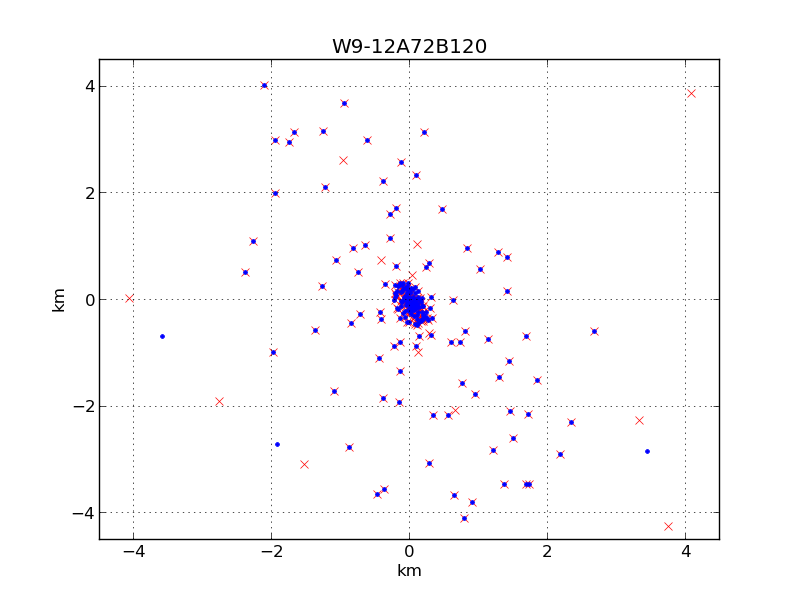
\includegraphics[width=0.150000\textwidth,trim= 0 .05cm 0 0.05cm]{{images/outer_core_SKA1W9-12A72B120}.png} &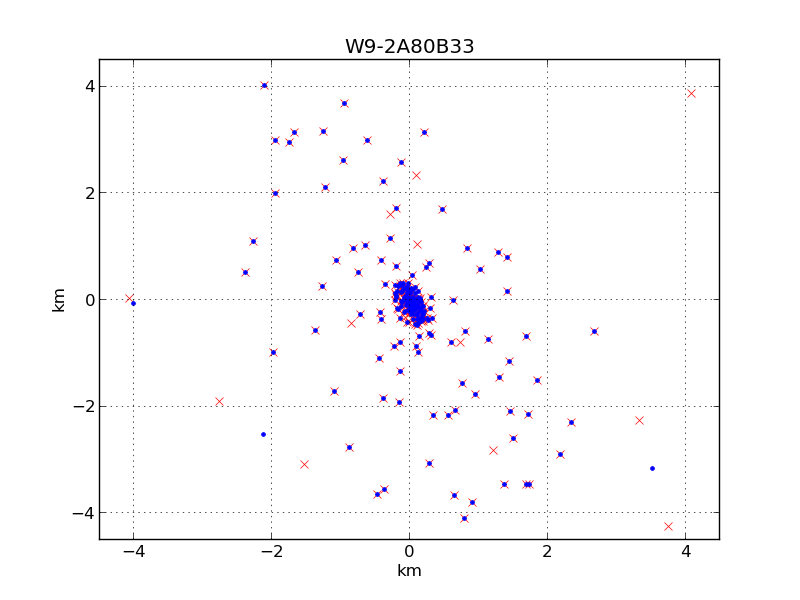
\includegraphics[width=0.150000\textwidth,trim= 0 .05cm 0 0.05cm]{{images/outer_core_SKA1W9-12A80B133}.png} 
 \\\end{tabular}}
 \caption{Antenna layouts, REF2 plotted as a reference (red crosses)}\label{fig:lay}
\end{figure}
% baseline distribution histograms

\begin{figure}[!htb]
\vspace{-.5cm}
 \tiny{%%% autogen
 \begin{tabular}{lllll}
\includegraphics[width=0.180000\textwidth,trim= 0 .05cm 0 0.05cm]{{}.images/hist*REF2png} &\includegraphics[width=0.180000\textwidth,trim= 0 .05cm 0 0.05cm]{{}.images/hist*W9-12A72png} &\includegraphics[width=0.180000\textwidth,trim= 0 .05cm 0 0.05cm]{{}.images/hist*W9-0A72png} &\includegraphics[width=0.180000\textwidth,trim= 0 .05cm 0 0.05cm]{{}.images/hist*SUR1png} &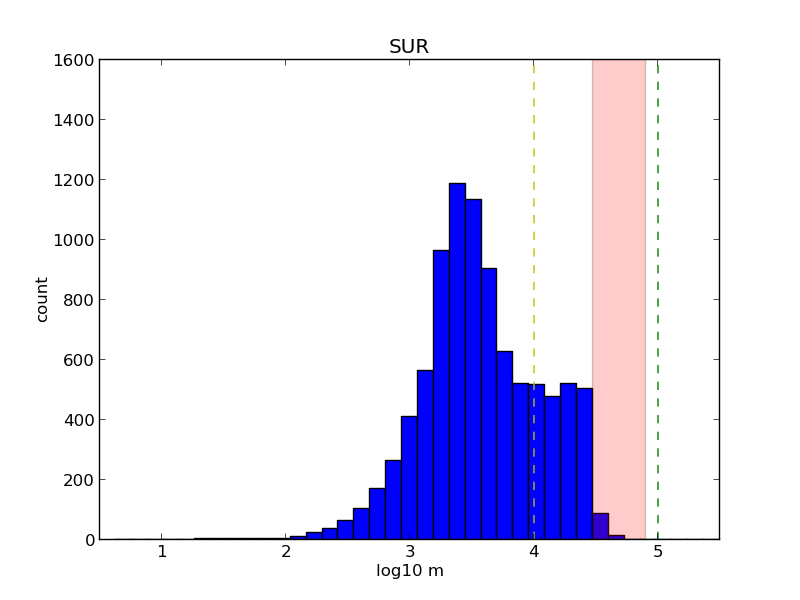
\includegraphics[width=0.180000\textwidth,trim= 0 .05cm 0 0.05cm]{{images/hist_SKASUR}.png} 
 \\ \hfill\end{tabular}}
 \caption{Baseline distribution with the uv-distance in $log_{10}$ km . Yellow and green dashed lines mark 10 and 120
kilometres respectively, and the pink strip represents baselines from 30-80km.}\label{fig:hist}
\end{figure}

% uv-coverage plots 
\begin{figure}[!htb]
 \tiny{%%% autogen
 \begin{tabular}{ccccc}
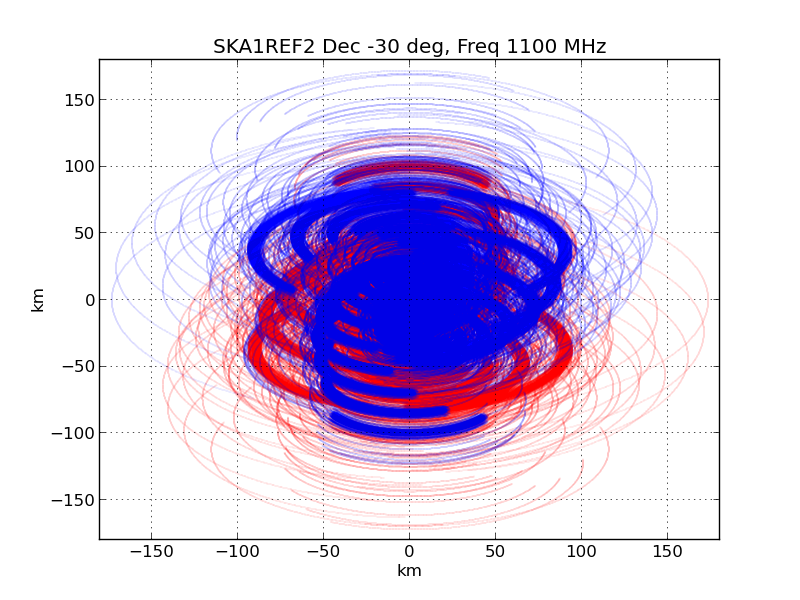
\includegraphics[width=0.180000\textwidth,trim= 0 .05cm 0 0.05cm]{{images/uvcov_SKA1REF2_-30_1100}.png} &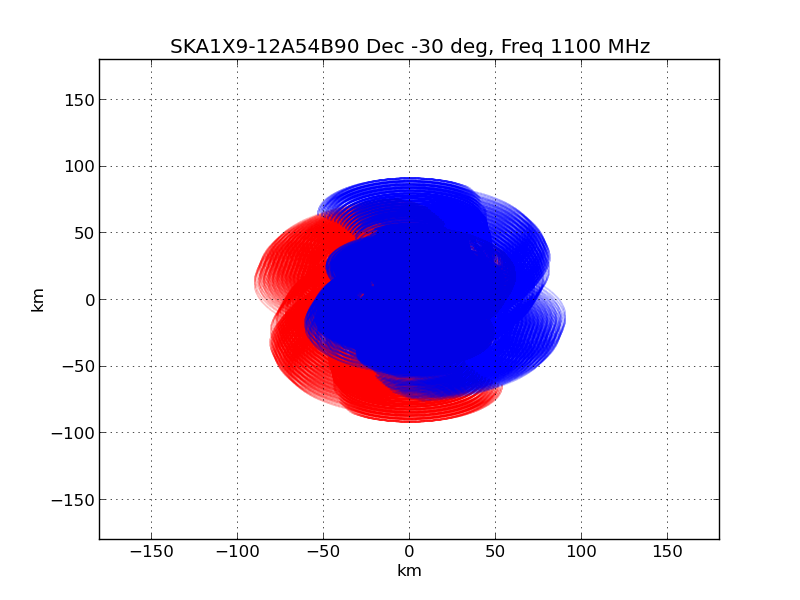
\includegraphics[width=0.180000\textwidth,trim= 0 .05cm 0 0.05cm]{{images/uvcov_SKA1X9-12A54B90_-30_1100}.png} &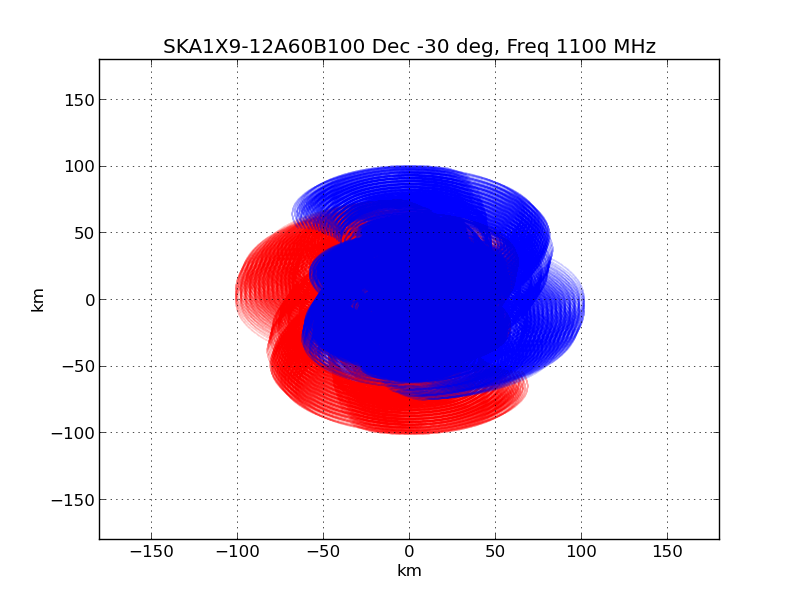
\includegraphics[width=0.180000\textwidth,trim= 0 .05cm 0 0.05cm]{{images/uvcov_SKA1X9-12A60B100_-30_1100}.png} &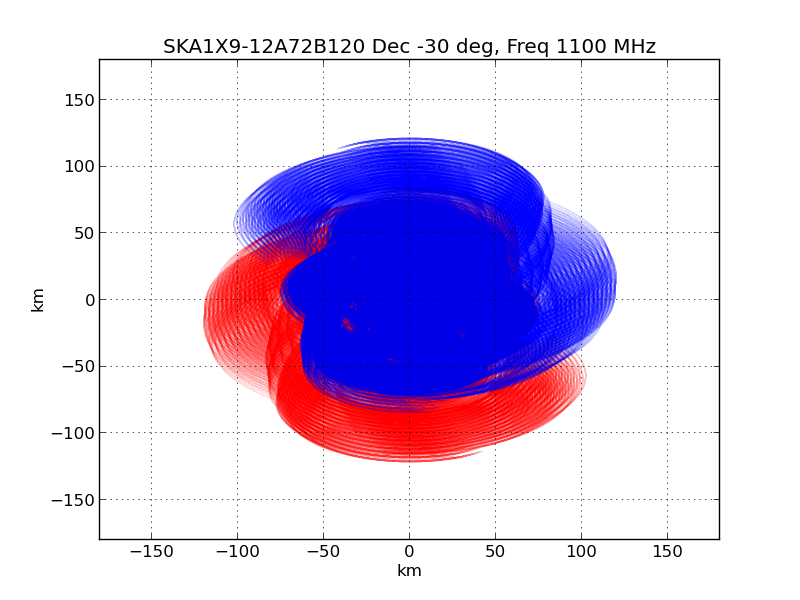
\includegraphics[width=0.180000\textwidth,trim= 0 .05cm 0 0.05cm]{{images/uvcov_SKA1X9-12A72B120_-30_1100}.png} &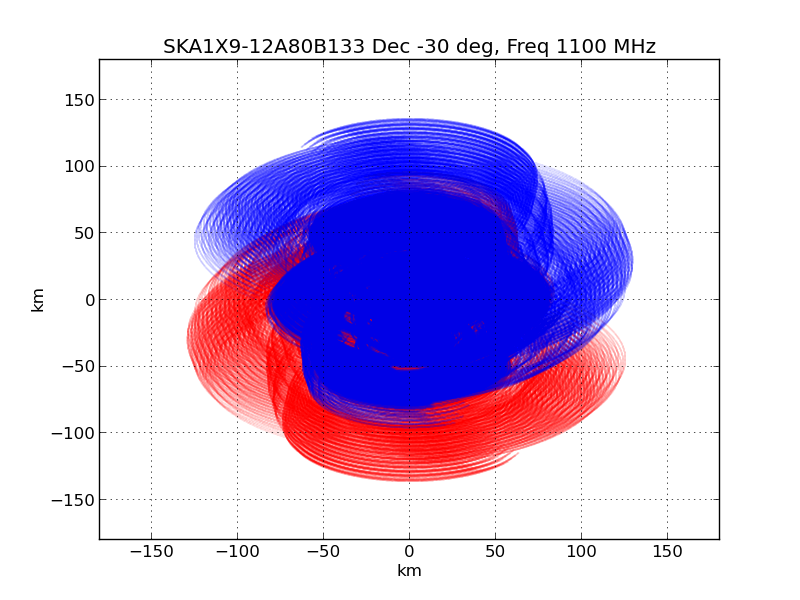
\includegraphics[width=0.180000\textwidth,trim= 0 .05cm 0 0.05cm]{{images/uvcov_SKA1X9-12A80B133_-30_1100}.png} 
 \\\end{tabular}}
 \caption{UV-Coverage for 8-hr tracks at 1.1 GHz (50MHz bandwidth) at declinations -50,-30,-10 for the different layouts. Blue
indicates uv-points, red indicates conjugate uv-points.}\label{fig:uvcov}
\end{figure}
\vspace{-.5cm}     
\section{The Experiment}\label{sec:exp}
\vspace{-.1cm}
Our aim is to investigate the scale-dependent sensitivity of the layouts described in the previous section. We use the
\texttt{makems} tool to make simulated measurement sets of 8hr tracks with a 60s integration time at declination -30 degrees
at frequencies of \{650, 800, 1100\}MHz with a single channel. The expected rms noise per real and imaginary part for each
visibility is calculated as $\sigma_{\text{vis}} = \text{SEFD}/\sqrt{2\Delta t\Delta \nu}$. We use the baseline design's {\it
system equivalent flux desnity} (SEFD) value of 400 corresponding to the 15 m dishes. We then fill the measurement set with random
Gaussian noise using the computed value of the noise for a given integration and bandwidth. We then use the (CASA-derived)
\texttt{lwimager} tool to make maps of the point spread function (PSF) as well as dirty maps of the noise using various weighting
schemes. Note that for uniform and robust weighting, a crucial parameter is the size of the uv-bin over which weights are
“uniformized”. By default this is determined from the full image size, but \texttt{lwimager} allows one to uniformize the weights
over bins corresponding to a user-defined field of view (FoV) instead. For these simulations uv-bins corresponding to a FoV of 10
arcmin were used. The following metrics were generated:\\ {\bf Note:} These metrics are generated at different angular scales,
this is done by applying an inner-taper\footnote{The weights for the taper are generated using a Butterworth function } to taper
out baselines that do not fall within a given resolution range, i.e., we only consider uv-points that correspond to a given
resolution.                                                                                         
\begin{itemize}
 \item PSF full width at half maximum (FWHM) size (mean of the FWHM dimensions). This was measured by making high-resolution
images of the PSF (0.05 arcsec
resolution), and fitting a Gaussian to the PSF. Note that for the highly non-Gaussian PSFs corresponding to natural and (some)
robust weighting schemes, the fit is very poor, so the size parameter becomes somewhat ill-defined (Table \ref{tab:psf_mean}).

 \item PSF symmetry (PSF size parameters are obtained as explained above). As a measure of PSF symmetry, we define 
$\text{PSF}_{sym}=1-\text{FWHM}_{min}/\text{FWHM}_{maj}$, then $\text{PSF}_{sym} = 0$ is perfect symmetry, and the symmetry
degenerates as $\text{PSF}_{sym}\,\,\, \rightarrow\,\,1$ (Table \ref{tab:psf_sym}).

 \item RMS pixel noise at different angular scales for a 166MHz wide band (Table \ref{tab:noise166}).
 
 \item SNR for a 10$\mu$Jy source at 1100MHz with a spectral index of -0.7 after 8hrs for a 166MHz band (Table \ref{tab:snr10}).
 \item Average SNR over frequencies 650, 800 and 1100MHz (166MHz band)
   after 8 hours, for a 10$\mu$Jy source at 1100MHz
with a spectral index of -0.7 (Table \ref{tab:snravg}). {$\overline{SNR10}=\sqrt{SNR10_{650}^2 + SNR10_{800}^2 +
SNR10_{1100}^2}$}.
 \item Hours required to reach a mean SNR of 10 (Table \ref{tab:hours}).
\end{itemize}

\section{Conclusions}\label{sec:conclusion}
\vspace{-.1cm}
The metrics we have used suggest that the science goals (at least those listed in the SKA1 Level-zero requirements) can be met by
a layout which covers significantly less space compared to the baseline layout. Some of these ``smaller'' layouts perform better
than the baseline layout at smaller scales, up to a 50\% improvement in terms of the noise properties, without compromising the
larger scales. This obviously presents an opportunity to reduce trenching and data transport costs. Moreover, bringing in the
dishes further out translates to a greater sensitivity on the relevant (to the science goals of SKA1-Mid) smaller scales, as can
be seen in Tables \ref{tab:noise166}-\ref{tab:hours}. Even more encouraging is the fact that this doesn't compromise the size or
the symmetry of the PSF as seen in Tables \ref{tab:psf_mean} and \ref{tab:psf_sym}.
\begin{thebibliography}{99}
 \bibitem{bd} \url{http://www.skatelescope.org/wp-content/uploads/2013/05/SKA-TEL-SKO-DD-001-1_BaselineDesign1.pdf}
 \bibitem{srd} \url{https://www.skatelescope.org/wp-content/uploads/2014/03/SKA-TEL_SCI-SKO-SRQ-001-1_Level_0_Requirements-1.pdf}
%  \bibitem{meqtrees} {Noordam, J. E., \& Smirnov, O. M. 2010, A\&A, 524, A61}
\end{thebibliography}
% Auto generated table
 \nopagebreak 
 \begin{table}[htp]
 \tiny{\subfloat[DEC=-30, natural weighting]{\begin{tabular}{|lccccc||ccccc||ccccc|} 
 \\ \cline{2-16} \multicolumn{1}{c}{ } & \multicolumn{5}{|c}{650MHz}  & \multicolumn{5}{c}{800MHz}  & \multicolumn{5}{c|}{1100MHz} \\ \cline{1-16} 
 resbin  &1 & 2 & 3 & 4 & 5 & 1 & 2 & 3 & 4 & 5 & 1 & 2 & 3 & 4 & 5 \\ \hline
SKA1REF2 & 0.65 \cellcolor{blue!18.00} & 1.34 \cellcolor{red!60.00} & 2.35 \cellcolor{green!18.00} & 3.37 \cellcolor{orange!60.00} & 797.29 \cellcolor{purple!60.00} & 0.60 \cellcolor{blue!18.00} & 1.33 \cellcolor{red!60.00} & 2.35 \cellcolor{green!38.65} & 3.34 \cellcolor{orange!32.44} & 790.58 \cellcolor{purple!58.08} & 0.59 \cellcolor{blue!43.54} & 1.33 \cellcolor{red!52.36} & 2.35 \cellcolor{green!35.14} & 3.35 \cellcolor{orange!36.02} & 759.20 \cellcolor{purple!18.00}\\ \hline 
SKA1X9-12A54B90 & 0.86 \cellcolor{blue!60.00} & 1.20 \cellcolor{red!23.77} & 2.36 \cellcolor{green!60.00} & 3.32 \cellcolor{orange!18.00} & 788.95 \cellcolor{purple!26.32} & 0.80 \cellcolor{blue!60.00} & 1.19 \cellcolor{red!18.00} & 2.34 \cellcolor{green!18.00} & 3.33 \cellcolor{orange!18.00} & 790.72 \cellcolor{purple!60.00} & 0.64 \cellcolor{blue!60.00} & 1.31 \cellcolor{red!18.00} & 2.35 \cellcolor{green!20.90} & 3.34 \cellcolor{orange!24.85} & 761.78 \cellcolor{purple!44.41}\\ \hline 
SKA1X9-12A60B100 & 0.84 \cellcolor{blue!55.85} & 1.18 \cellcolor{red!18.00} & 2.35 \cellcolor{green!39.48} & 3.36 \cellcolor{orange!48.37} & 789.63 \cellcolor{purple!29.05} & 0.75 \cellcolor{blue!48.82} & 1.26 \cellcolor{red!38.80} & 2.34 \cellcolor{green!24.93} & 3.34 \cellcolor{orange!19.87} & 788.41 \cellcolor{purple!27.83} & 0.60 \cellcolor{blue!46.34} & 1.34 \cellcolor{red!55.52} & 2.36 \cellcolor{green!58.31} & 3.37 \cellcolor{orange!60.00} & 760.33 \cellcolor{purple!29.63}\\ \hline 
SKA1X9-12A72B120 & 0.76 \cellcolor{blue!40.51} & 1.26 \cellcolor{red!40.49} & 2.35 \cellcolor{green!33.75} & 3.36 \cellcolor{orange!50.68} & 786.89 \cellcolor{purple!18.00} & 0.66 \cellcolor{blue!30.68} & 1.31 \cellcolor{red!53.90} & 2.34 \cellcolor{green!28.61} & 3.33 \cellcolor{orange!19.12} & 787.70 \cellcolor{purple!18.00} & 0.52 \cellcolor{blue!24.31} & 1.34 \cellcolor{red!60.00} & 2.36 \cellcolor{green!60.00} & 3.36 \cellcolor{orange!54.14} & 761.09 \cellcolor{purple!37.39}\\ \hline 
SKA1X9-12A80B133 & 0.71 \cellcolor{blue!29.63} & 1.29 \cellcolor{red!46.64} & 2.35 \cellcolor{green!30.89} & 3.34 \cellcolor{orange!31.29} & 788.81 \cellcolor{purple!25.73} & 0.61 \cellcolor{blue!20.31} & 1.33 \cellcolor{red!59.47} & 2.37 \cellcolor{green!60.00} & 3.36 \cellcolor{orange!60.00} & 789.88 \cellcolor{purple!48.31} & 0.50 \cellcolor{blue!18.00} & 1.32 \cellcolor{red!36.43} & 2.34 \cellcolor{green!18.00} & 3.33 \cellcolor{orange!18.00} & 763.30 \cellcolor{purple!60.00}\\ \hline 
\end{tabular}}
\vspace{-0.300000cm}
\hspace{1cm} 
\subfloat[DEC=-30, robust-2 weighting ]{\begin{tabular}{|lccccc||ccccc||ccccc|} 
 \\ \cline{2-16} \multicolumn{1}{c}{ } & \multicolumn{5}{|c}{650MHz}  & \multicolumn{5}{c}{800MHz}  & \multicolumn{5}{c|}{1100MHz} \\ \cline{1-16} 
 resbin  &1 & 2 & 3 & 4 & 5 & 1 & 2 & 3 & 4 & 5 & 1 & 2 & 3 & 4 & 5 \\ \hline
SKA1REF2 & 0.71 \cellcolor{blue!29.98} & 1.21 \cellcolor{red!60.00} & 2.24 \cellcolor{green!42.92} & 3.26 \cellcolor{orange!58.03} & 737.52 \cellcolor{purple!60.00} & 0.60 \cellcolor{blue!25.71} & 1.19 \cellcolor{red!60.00} & 2.24 \cellcolor{green!55.48} & 3.24 \cellcolor{orange!18.00} & 789.76 \cellcolor{purple!47.02} & 0.51 \cellcolor{blue!35.29} & 1.18 \cellcolor{red!60.00} & 2.24 \cellcolor{green!47.30} & 3.25 \cellcolor{orange!20.04} & 757.10 \cellcolor{purple!18.00}\\ \hline 
SKA1X9-12A54B90 & 0.87 \cellcolor{blue!60.00} & 1.19 \cellcolor{red!49.31} & 2.23 \cellcolor{green!18.00} & 3.25 \cellcolor{orange!39.66} & 730.57 \cellcolor{purple!27.92} & 0.71 \cellcolor{blue!60.00} & 1.14 \cellcolor{red!21.71} & 2.23 \cellcolor{green!18.00} & 3.26 \cellcolor{orange!60.00} & 790.68 \cellcolor{purple!60.00} & 0.55 \cellcolor{blue!60.00} & 1.15 \cellcolor{red!18.00} & 2.23 \cellcolor{green!18.00} & 3.26 \cellcolor{orange!60.00} & 760.85 \cellcolor{purple!48.38}\\ \hline 
SKA1X9-12A60B100 & 0.80 \cellcolor{blue!46.74} & 1.15 \cellcolor{red!28.51} & 2.24 \cellcolor{green!51.46} & 3.25 \cellcolor{orange!18.00} & 728.67 \cellcolor{purple!19.10} & 0.66 \cellcolor{blue!44.02} & 1.13 \cellcolor{red!18.00} & 2.24 \cellcolor{green!33.35} & 3.25 \cellcolor{orange!53.70} & 788.24 \cellcolor{purple!25.32} & 0.54 \cellcolor{blue!51.05} & 1.16 \cellcolor{red!34.05} & 2.24 \cellcolor{green!60.00} & 3.25 \cellcolor{orange!28.19} & 759.63 \cellcolor{purple!38.51}\\ \hline 
SKA1X9-12A72B120 & 0.70 \cellcolor{blue!27.88} & 1.13 \cellcolor{red!18.00} & 2.25 \cellcolor{green!60.00} & 3.25 \cellcolor{orange!25.22} & 728.43 \cellcolor{purple!18.00} & 0.59 \cellcolor{blue!23.48} & 1.16 \cellcolor{red!36.56} & 2.24 \cellcolor{green!22.97} & 3.25 \cellcolor{orange!49.15} & 787.72 \cellcolor{purple!18.00} & 0.52 \cellcolor{blue!35.67} & 1.17 \cellcolor{red!55.05} & 2.24 \cellcolor{green!58.05} & 3.25 \cellcolor{orange!18.00} & 760.45 \cellcolor{purple!45.13}\\ \hline 
SKA1X9-12A80B133 & 0.65 \cellcolor{blue!18.00} & 1.14 \cellcolor{red!20.99} & 2.24 \cellcolor{green!51.69} & 3.26 \cellcolor{orange!60.00} & 730.10 \cellcolor{purple!25.73} & 0.57 \cellcolor{blue!18.00} & 1.17 \cellcolor{red!45.98} & 2.24 \cellcolor{green!60.00} & 3.25 \cellcolor{orange!46.00} & 789.76 \cellcolor{purple!47.00} & 0.49 \cellcolor{blue!18.00} & 1.17 \cellcolor{red!51.12} & 2.23 \cellcolor{green!27.12} & 3.26 \cellcolor{orange!56.33} & 762.28 \cellcolor{purple!60.00}\\ \hline 
\end{tabular}}
\vspace{-0.300000cm}
\hspace{1cm} 

\vspace{.25cm}
\caption{FWHM PSF sizes (in arcseconds) for the different layouts at different angular scales. These values are generated at 650, 800 and 1100MHz, for angular scales \{0.4-1, 1-2, 2-3, 3-4, 600-3600\} arcsec and are labeled {\it resbin} \{1, 2, 3, 4, 5\} respectively. This is done for natural and robust-2 weighting at declination -30 degrees. For each column, the intensity of the color increases with the value.}\label{tab:psf_mean}}
 \end{table}

% Auto generated table
 \nopagebreak 
 \begin{table}[htp]
 \tiny{\subfloat[DEC=-30, natural weighting]{\begin{tabular}{|lccccc||ccccc||ccccc|} 
 \\ \cline{2-16} \multicolumn{1}{c}{ } & \multicolumn{5}{|c}{650MHz}  & \multicolumn{5}{c}{800MHz}  & \multicolumn{5}{c|}{1100MHz} \\ \cline{1-16} 
 resbin  &1 & 2 & 3 & 4 & 5 & 1 & 2 & 3 & 4 & 5 & 1 & 2 & 3 & 4 & 5 \\ \hline
SKA1REF2 & 0.13 \cellcolor{blue!18.00} & 0.07 \cellcolor{red!44.25} & 0.08 \cellcolor{green!60.00} & 0.06 \cellcolor{orange!39.00} & 0.02 \cellcolor{purple!18.00} & 0.09 \cellcolor{blue!18.00} & 0.08 \cellcolor{red!54.75} & 0.06 \cellcolor{green!18.00} & 0.08 \cellcolor{orange!49.50} & 0.03 \cellcolor{purple!60.00} & 0.06 \cellcolor{blue!18.00} & 0.08 \cellcolor{red!60.00} & 0.06 \cellcolor{green!28.50} & 0.05 \cellcolor{orange!49.50} & 0.07 \cellcolor{purple!60.00}\\ \hline 
SKA1X9-12A54B90 & 0.20 \cellcolor{blue!60.00} & 0.08 \cellcolor{red!49.50} & 0.06 \cellcolor{green!39.00} & 0.05 \cellcolor{orange!28.50} & 0.03 \cellcolor{purple!39.00} & 0.17 \cellcolor{blue!60.00} & 0.05 \cellcolor{red!39.00} & 0.08 \cellcolor{green!60.00} & 0.05 \cellcolor{orange!18.00} & 0.03 \cellcolor{purple!60.00} & 0.11 \cellcolor{blue!60.00} & 0.05 \cellcolor{red!18.00} & 0.08 \cellcolor{green!49.50} & 0.06 \cellcolor{orange!60.00} & 0.04 \cellcolor{purple!28.50}\\ \hline 
SKA1X9-12A60B100 & 0.19 \cellcolor{blue!54.00} & 0.02 \cellcolor{red!18.00} & 0.04 \cellcolor{green!18.00} & 0.08 \cellcolor{orange!60.00} & 0.03 \cellcolor{purple!39.00} & 0.14 \cellcolor{blue!44.25} & 0.09 \cellcolor{red!60.00} & 0.07 \cellcolor{green!39.00} & 0.09 \cellcolor{orange!60.00} & 0.02 \cellcolor{purple!18.00} & 0.11 \cellcolor{blue!60.00} & 0.06 \cellcolor{red!32.00} & 0.05 \cellcolor{green!18.00} & 0.06 \cellcolor{orange!60.00} & 0.03 \cellcolor{purple!18.00}\\ \hline 
SKA1X9-12A72B120 & 0.15 \cellcolor{blue!30.00} & 0.10 \cellcolor{red!60.00} & 0.04 \cellcolor{green!18.00} & 0.08 \cellcolor{orange!60.00} & 0.03 \cellcolor{purple!39.00} & 0.12 \cellcolor{blue!33.75} & 0.01 \cellcolor{red!18.00} & 0.07 \cellcolor{green!39.00} & 0.09 \cellcolor{orange!60.00} & 0.02 \cellcolor{purple!18.00} & 0.11 \cellcolor{blue!60.00} & 0.06 \cellcolor{red!32.00} & 0.05 \cellcolor{green!18.00} & 0.06 \cellcolor{orange!60.00} & 0.03 \cellcolor{purple!18.00}\\ \hline 
SKA1X9-12A80B133 & 0.13 \cellcolor{blue!18.00} & 0.03 \cellcolor{red!23.25} & 0.06 \cellcolor{green!39.00} & 0.04 \cellcolor{orange!18.00} & 0.04 \cellcolor{purple!60.00} & 0.11 \cellcolor{blue!28.50} & 0.05 \cellcolor{red!39.00} & 0.06 \cellcolor{green!18.00} & 0.06 \cellcolor{orange!28.50} & 0.02 \cellcolor{purple!18.00} & 0.06 \cellcolor{blue!18.00} & 0.06 \cellcolor{red!32.00} & 0.09 \cellcolor{green!60.00} & 0.02 \cellcolor{orange!18.00} & 0.03 \cellcolor{purple!18.00}\\ \hline 
\end{tabular}}
\vspace{-0.300000cm}
\hspace{1cm} 
\subfloat[DEC=-30, robust-2 weighting ]{\begin{tabular}{|lccccc||ccccc||ccccc|} 
 \\ \cline{2-16} \multicolumn{1}{c}{ } & \multicolumn{5}{|c}{650MHz}  & \multicolumn{5}{c}{800MHz}  & \multicolumn{5}{c|}{1100MHz} \\ \cline{1-16} 
 resbin  &1 & 2 & 3 & 4 & 5 & 1 & 2 & 3 & 4 & 5 & 1 & 2 & 3 & 4 & 5 \\ \hline
SKA1REF2 & 0.12 \cellcolor{blue!60.00} & 0.04 \cellcolor{red!60.00} & 0.02 \cellcolor{green!60.00} & 0.01 \cellcolor{orange!60.00} & 0.05 \cellcolor{purple!60.00} & 0.11 \cellcolor{blue!60.00} & 0.03 \cellcolor{red!60.00} & 0.00 \cellcolor{green!18.00} & 0.01 \cellcolor{orange!60.00} & 0.03 \cellcolor{purple!60.00} & 0.07 \cellcolor{blue!60.00} & 0.02 \cellcolor{red!60.00} & 0.00 \cellcolor{green!18.00} & 0.01 \cellcolor{orange!60.00} & 0.07 \cellcolor{purple!60.00}\\ \hline 
SKA1X9-12A54B90 & 0.10 \cellcolor{blue!18.00} & 0.03 \cellcolor{red!49.50} & 0.01 \cellcolor{green!39.00} & 0.00 \cellcolor{orange!18.00} & 0.03 \cellcolor{purple!18.00} & 0.10 \cellcolor{blue!49.50} & 0.02 \cellcolor{red!46.00} & 0.00 \cellcolor{green!18.00} & 0.00 \cellcolor{orange!18.00} & 0.03 \cellcolor{purple!60.00} & 0.07 \cellcolor{blue!60.00} & 0.01 \cellcolor{red!18.00} & 0.01 \cellcolor{green!60.00} & 0.00 \cellcolor{orange!18.00} & 0.04 \cellcolor{purple!28.50}\\ \hline 
SKA1X9-12A60B100 & 0.10 \cellcolor{blue!18.00} & 0.03 \cellcolor{red!49.50} & 0.00 \cellcolor{green!18.00} & 0.01 \cellcolor{orange!60.00} & 0.04 \cellcolor{purple!39.00} & 0.10 \cellcolor{blue!49.50} & 0.01 \cellcolor{red!32.00} & 0.01 \cellcolor{green!60.00} & 0.00 \cellcolor{orange!18.00} & 0.02 \cellcolor{purple!18.00} & 0.06 \cellcolor{blue!39.00} & 0.01 \cellcolor{red!18.00} & 0.00 \cellcolor{green!18.00} & 0.01 \cellcolor{orange!60.00} & 0.03 \cellcolor{purple!18.00}\\ \hline 
SKA1X9-12A72B120 & 0.11 \cellcolor{blue!39.00} & 0.01 \cellcolor{red!28.50} & 0.01 \cellcolor{green!39.00} & 0.01 \cellcolor{orange!60.00} & 0.03 \cellcolor{purple!18.00} & 0.09 \cellcolor{blue!39.00} & 0.01 \cellcolor{red!32.00} & 0.01 \cellcolor{green!60.00} & 0.00 \cellcolor{orange!18.00} & 0.02 \cellcolor{purple!18.00} & 0.05 \cellcolor{blue!18.00} & 0.01 \cellcolor{red!18.00} & 0.00 \cellcolor{green!18.00} & 0.01 \cellcolor{orange!60.00} & 0.03 \cellcolor{purple!18.00}\\ \hline 
SKA1X9-12A80B133 & 0.10 \cellcolor{blue!18.00} & 0.00 \cellcolor{red!18.00} & 0.01 \cellcolor{green!39.00} & 0.00 \cellcolor{orange!18.00} & 0.03 \cellcolor{purple!18.00} & 0.07 \cellcolor{blue!18.00} & 0.00 \cellcolor{red!18.00} & 0.00 \cellcolor{green!18.00} & 0.01 \cellcolor{orange!60.00} & 0.02 \cellcolor{purple!18.00} & 0.06 \cellcolor{blue!39.00} & 0.02 \cellcolor{red!60.00} & 0.01 \cellcolor{green!60.00} & 0.00 \cellcolor{orange!18.00} & 0.03 \cellcolor{purple!18.00}\\ \hline 
\end{tabular}}
\vspace{-0.300000cm}
\hspace{1cm} 

\vspace{.25cm}
\caption{PSF symmetry (see \autoref{sec:exp})  for the different layouts at different scales. These values are generate at 650, 800 and 1100MHz, for angular scales \{0.4-1, 1-2, 2-3, 3-4, 600-3600\} arcsec labeled as {\it resbin} \{1, 2, 3, 4, 5\} respectively. This is done for natural and robust-2 weighting at declination -30 degrees. For each column, the intensity of the color increases with the value.}\label{tab:psf_sym}}
 \end{table}

% Auto generated table
 \nopagebreak 
 \begin{table}[htp]
 \tiny{\subfloat[DEC=-30, natural weighting]{\begin{tabular}{|lccccc||ccccc||ccccc|} 
 \\ \cline{2-16} \multicolumn{1}{c}{ } & \multicolumn{5}{|c}{650MHz}  & \multicolumn{5}{c}{800MHz}  & \multicolumn{5}{c|}{1100MHz} \\ \cline{1-16} 
 resbin  &1 & 2 & 3 & 4 & 5 & 1 & 2 & 3 & 4 & 5 & 1 & 2 & 3 & 4 & 5 \\ \hline
SKA1REF2 & 1.50 \cellcolor{blue!60.00} & 1.60 \cellcolor{red!60.00} & 2.10 \cellcolor{green!18.00} & 2.60 \cellcolor{orange!18.00} & 5.60 \cellcolor{purple!18.00} & 1.40 \cellcolor{blue!60.00} & 1.60 \cellcolor{red!49.50} & 2.20 \cellcolor{green!18.00} & 2.60 \cellcolor{orange!18.00} & 7.10 \cellcolor{purple!18.00} & 1.40 \cellcolor{blue!60.00} & 1.60 \cellcolor{red!18.00} & 2.20 \cellcolor{green!18.00} & 2.60 \cellcolor{orange!18.00} & 10.00 \cellcolor{purple!18.00}\\ \hline 
SKA1X9-12A54B90 & 1.40 \cellcolor{blue!52.88} & 0.98 \cellcolor{red!18.00} & 2.20 \cellcolor{green!32.00} & 2.80 \cellcolor{orange!39.00} & 5.90 \cellcolor{purple!60.00} & 1.00 \cellcolor{blue!27.06} & 1.30 \cellcolor{red!18.00} & 2.20 \cellcolor{green!18.00} & 2.90 \cellcolor{orange!49.50} & 7.50 \cellcolor{purple!60.00} & 0.91 \cellcolor{blue!20.42} & 1.70 \cellcolor{red!39.00} & 2.30 \cellcolor{green!39.00} & 2.70 \cellcolor{orange!28.50} & 11.00 \cellcolor{purple!60.00}\\ \hline 
SKA1X9-12A60B100 & 1.20 \cellcolor{blue!38.64} & 1.10 \cellcolor{red!26.13} & 2.30 \cellcolor{green!46.00} & 2.70 \cellcolor{orange!28.50} & 5.90 \cellcolor{purple!60.00} & 0.96 \cellcolor{blue!23.76} & 1.50 \cellcolor{red!39.00} & 2.30 \cellcolor{green!39.00} & 2.70 \cellcolor{orange!28.50} & 7.50 \cellcolor{purple!60.00} & 0.90 \cellcolor{blue!19.62} & 1.70 \cellcolor{red!39.00} & 2.40 \cellcolor{green!60.00} & 2.80 \cellcolor{orange!39.00} & 11.00 \cellcolor{purple!60.00}\\ \hline 
SKA1X9-12A72B120 & 0.95 \cellcolor{blue!20.85} & 1.50 \cellcolor{red!53.23} & 2.40 \cellcolor{green!60.00} & 2.80 \cellcolor{orange!39.00} & 5.90 \cellcolor{purple!60.00} & 0.93 \cellcolor{blue!21.29} & 1.70 \cellcolor{red!60.00} & 2.40 \cellcolor{green!60.00} & 2.70 \cellcolor{orange!28.50} & 7.50 \cellcolor{purple!60.00} & 0.88 \cellcolor{blue!18.00} & 1.80 \cellcolor{red!60.00} & 2.40 \cellcolor{green!60.00} & 2.90 \cellcolor{orange!49.50} & 11.00 \cellcolor{purple!60.00}\\ \hline 
SKA1X9-12A80B133 & 0.91 \cellcolor{blue!18.00} & 1.50 \cellcolor{red!53.23} & 2.20 \cellcolor{green!32.00} & 3.00 \cellcolor{orange!60.00} & 5.90 \cellcolor{purple!60.00} & 0.89 \cellcolor{blue!18.00} & 1.70 \cellcolor{red!60.00} & 2.40 \cellcolor{green!60.00} & 3.00 \cellcolor{orange!60.00} & 7.50 \cellcolor{purple!60.00} & 0.92 \cellcolor{blue!21.23} & 1.70 \cellcolor{red!39.00} & 2.30 \cellcolor{green!39.00} & 3.00 \cellcolor{orange!60.00} & 11.00 \cellcolor{purple!60.00}\\ \hline 
\end{tabular}}
\vspace{-0.300000cm}
\hspace{1cm} 
\subfloat[DEC=-30, robust-2 weighting ]{\begin{tabular}{|lccccc||ccccc||ccccc|} 
 \\ \cline{2-16} \multicolumn{1}{c}{ } & \multicolumn{5}{|c}{650MHz}  & \multicolumn{5}{c}{800MHz}  & \multicolumn{5}{c|}{1100MHz} \\ \cline{1-16} 
 resbin  &1 & 2 & 3 & 4 & 5 & 1 & 2 & 3 & 4 & 5 & 1 & 2 & 3 & 4 & 5 \\ \hline
SKA1REF2 & 1.70 \cellcolor{blue!60.00} & 2.00 \cellcolor{red!60.00} & 2.60 \cellcolor{green!32.00} & 2.70 \cellcolor{orange!18.00} & 5.40 \cellcolor{purple!18.00} & 1.60 \cellcolor{blue!60.00} & 2.10 \cellcolor{red!60.00} & 2.50 \cellcolor{green!18.00} & 2.60 \cellcolor{orange!18.00} & 7.10 \cellcolor{purple!18.00} & 1.70 \cellcolor{blue!60.00} & 2.10 \cellcolor{red!39.00} & 2.30 \cellcolor{green!18.00} & 2.50 \cellcolor{orange!18.00} & 10.00 \cellcolor{purple!18.00}\\ \hline 
SKA1X9-12A54B90 & 1.70 \cellcolor{blue!60.00} & 1.30 \cellcolor{red!18.00} & 2.50 \cellcolor{green!18.00} & 2.90 \cellcolor{orange!39.00} & 5.70 \cellcolor{purple!49.50} & 1.60 \cellcolor{blue!60.00} & 1.30 \cellcolor{red!18.00} & 2.50 \cellcolor{green!18.00} & 2.80 \cellcolor{orange!39.00} & 7.50 \cellcolor{purple!60.00} & 1.60 \cellcolor{blue!51.60} & 1.90 \cellcolor{red!18.00} & 2.40 \cellcolor{green!28.50} & 2.60 \cellcolor{orange!28.50} & 11.00 \cellcolor{purple!60.00}\\ \hline 
SKA1X9-12A60B100 & 1.60 \cellcolor{blue!49.50} & 1.30 \cellcolor{red!18.00} & 2.60 \cellcolor{green!32.00} & 2.90 \cellcolor{orange!39.00} & 5.80 \cellcolor{purple!60.00} & 1.50 \cellcolor{blue!46.00} & 1.50 \cellcolor{red!28.50} & 2.60 \cellcolor{green!39.00} & 2.90 \cellcolor{orange!49.50} & 7.50 \cellcolor{purple!60.00} & 1.50 \cellcolor{blue!43.20} & 2.00 \cellcolor{red!28.50} & 2.40 \cellcolor{green!28.50} & 2.60 \cellcolor{orange!28.50} & 11.00 \cellcolor{purple!60.00}\\ \hline 
SKA1X9-12A72B120 & 1.40 \cellcolor{blue!28.50} & 1.50 \cellcolor{red!30.00} & 2.80 \cellcolor{green!60.00} & 3.10 \cellcolor{orange!60.00} & 5.70 \cellcolor{purple!49.50} & 1.40 \cellcolor{blue!32.00} & 1.90 \cellcolor{red!49.50} & 2.70 \cellcolor{green!60.00} & 3.00 \cellcolor{orange!60.00} & 7.50 \cellcolor{purple!60.00} & 1.30 \cellcolor{blue!26.40} & 2.20 \cellcolor{red!49.50} & 2.60 \cellcolor{green!49.50} & 2.80 \cellcolor{orange!49.50} & 11.00 \cellcolor{purple!60.00}\\ \hline 
SKA1X9-12A80B133 & 1.30 \cellcolor{blue!18.00} & 1.70 \cellcolor{red!42.00} & 2.80 \cellcolor{green!60.00} & 3.10 \cellcolor{orange!60.00} & 5.70 \cellcolor{purple!49.50} & 1.30 \cellcolor{blue!18.00} & 2.10 \cellcolor{red!60.00} & 2.70 \cellcolor{green!60.00} & 3.00 \cellcolor{orange!60.00} & 7.50 \cellcolor{purple!60.00} & 1.20 \cellcolor{blue!18.00} & 2.30 \cellcolor{red!60.00} & 2.70 \cellcolor{green!60.00} & 2.90 \cellcolor{orange!60.00} & 11.00 \cellcolor{purple!60.00}\\ \hline 
\end{tabular}}
\vspace{-0.300000cm}
\hspace{1cm} 

\vspace{.25cm}
\caption{Noise (in $\mu$Jy) for a 166MHz band after an 8hr synthesis with a 60s integration for the different layouts at different angular scales. These values are generated at 650, 800 and 1100 MHz, at angular scales \{0.4-1, 1-2, 2-3, 3-4, 600-3600\} arcsec and are labeled {\it resbin} \{1, 2, 3, 4, 5\} respectively. This is done for natural and robust-2 weighting at declination -30 degrees. For each column, the intensity of the color increases with the value.}\label{tab:noise166}}
 \end{table}

% Auto generated table
 \nopagebreak 
 \begin{table}[htp]
 \tiny{\subfloat[DEC=-30, natural weighting]{\begin{tabular}{|lccccc||ccccc||ccccc|} 
 \\ \cline{2-16} \multicolumn{1}{c}{ } & \multicolumn{5}{|c}{650MHz}  & \multicolumn{5}{c}{800MHz}  & \multicolumn{5}{c|}{1100MHz} \\ \cline{1-16} 
 resbin  &1 & 2 & 3 & 4 & 5 & 1 & 2 & 3 & 4 & 5 & 1 & 2 & 3 & 4 & 5 \\ \hline
SKA1REF2 & 9.52 \cellcolor{blue!18.00} & 8.85 \cellcolor{red!18.00} & 6.74 \cellcolor{green!60.00} & 5.51 \cellcolor{orange!60.00} & 2.57 \cellcolor{purple!60.00} & 8.86 \cellcolor{blue!18.00} & 7.65 \cellcolor{red!23.29} & 5.60 \cellcolor{green!50.57} & 4.79 \cellcolor{orange!60.00} & 1.76 \cellcolor{purple!60.00} & 7.14 \cellcolor{blue!18.00} & 6.11 \cellcolor{red!60.00} & 4.53 \cellcolor{green!60.00} & 3.86 \cellcolor{orange!60.00} & 1.00 \cellcolor{purple!60.00}\\ \hline 
SKA1X9-12A54B90 & 10.04 \cellcolor{blue!21.46} & 14.82 \cellcolor{red!60.00} & 6.59 \cellcolor{green!50.16} & 5.15 \cellcolor{orange!37.09} & 2.47 \cellcolor{purple!27.69} & 12.30 \cellcolor{blue!46.00} & 9.94 \cellcolor{red!60.00} & 5.71 \cellcolor{green!60.00} & 4.30 \cellcolor{orange!23.89} & 1.66 \cellcolor{purple!18.00} & 11.02 \cellcolor{blue!56.25} & 6.00 \cellcolor{red!48.73} & 4.32 \cellcolor{green!37.38} & 3.73 \cellcolor{orange!50.59} & 0.92 \cellcolor{purple!18.00}\\ \hline 
SKA1X9-12A60B100 & 12.35 \cellcolor{blue!36.84} & 13.26 \cellcolor{red!49.03} & 6.28 \cellcolor{green!29.81} & 5.29 \cellcolor{orange!46.00} & 2.44 \cellcolor{purple!18.00} & 12.99 \cellcolor{blue!51.62} & 8.46 \cellcolor{red!36.27} & 5.37 \cellcolor{green!30.86} & 4.56 \cellcolor{orange!43.05} & 1.67 \cellcolor{purple!22.20} & 11.13 \cellcolor{blue!57.34} & 5.87 \cellcolor{red!35.41} & 4.14 \cellcolor{green!18.00} & 3.62 \cellcolor{orange!42.62} & 0.94 \cellcolor{purple!28.50}\\ \hline 
SKA1X9-12A72B120 & 15.18 \cellcolor{blue!55.67} & 9.96 \cellcolor{red!25.81} & 6.10 \cellcolor{green!18.00} & 5.18 \cellcolor{orange!39.00} & 2.46 \cellcolor{purple!24.46} & 13.47 \cellcolor{blue!55.52} & 7.42 \cellcolor{red!19.60} & 5.22 \cellcolor{green!18.00} & 4.57 \cellcolor{orange!43.79} & 1.66 \cellcolor{purple!18.00} & 11.40 \cellcolor{blue!60.00} & 5.70 \cellcolor{red!18.00} & 4.14 \cellcolor{green!18.00} & 3.49 \cellcolor{orange!33.21} & 0.94 \cellcolor{purple!28.50}\\ \hline 
SKA1X9-12A80B133 & 15.83 \cellcolor{blue!60.00} & 9.43 \cellcolor{red!22.08} & 6.44 \cellcolor{green!40.31} & 4.85 \cellcolor{orange!18.00} & 2.45 \cellcolor{purple!21.23} & 14.02 \cellcolor{blue!60.00} & 7.32 \cellcolor{red!18.00} & 5.30 \cellcolor{green!24.86} & 4.22 \cellcolor{orange!18.00} & 1.67 \cellcolor{purple!22.20} & 10.82 \cellcolor{blue!54.28} & 5.72 \cellcolor{red!20.05} & 4.28 \cellcolor{green!33.08} & 3.28 \cellcolor{orange!18.00} & 0.92 \cellcolor{purple!18.00}\\ \hline 
\end{tabular}}
\vspace{-0.300000cm}
\hspace{1cm} 
\subfloat[DEC=-30, robust-2 weighting ]{\begin{tabular}{|lccccc||ccccc||ccccc|} 
 \\ \cline{2-16} \multicolumn{1}{c}{ } & \multicolumn{5}{|c}{650MHz}  & \multicolumn{5}{c}{800MHz}  & \multicolumn{5}{c|}{1100MHz} \\ \cline{1-16} 
 resbin  &1 & 2 & 3 & 4 & 5 & 1 & 2 & 3 & 4 & 5 & 1 & 2 & 3 & 4 & 5 \\ \hline
SKA1REF2 & 8.74 \cellcolor{blue!19.77} & 7.07 \cellcolor{red!18.00} & 5.62 \cellcolor{green!49.50} & 5.29 \cellcolor{orange!60.00} & 2.66 \cellcolor{purple!60.00} & 7.60 \cellcolor{blue!18.00} & 5.91 \cellcolor{red!18.00} & 5.03 \cellcolor{green!60.00} & 4.74 \cellcolor{orange!60.00} & 1.75 \cellcolor{purple!60.00} & 5.87 \cellcolor{blue!18.00} & 4.66 \cellcolor{red!30.38} & 4.34 \cellcolor{green!60.00} & 4.05 \cellcolor{orange!60.00} & 0.99 \cellcolor{purple!60.00}\\ \hline 
SKA1X9-12A54B90 & 8.65 \cellcolor{blue!18.00} & 11.24 \cellcolor{red!57.18} & 5.75 \cellcolor{green!60.00} & 5.02 \cellcolor{orange!41.10} & 2.52 \cellcolor{purple!27.33} & 7.60 \cellcolor{blue!18.00} & 9.61 \cellcolor{red!60.00} & 4.96 \cellcolor{green!53.61} & 4.50 \cellcolor{orange!43.20} & 1.66 \cellcolor{purple!18.00} & 6.29 \cellcolor{blue!25.98} & 5.33 \cellcolor{red!60.00} & 4.10 \cellcolor{green!42.32} & 3.81 \cellcolor{orange!43.74} & 0.92 \cellcolor{purple!18.00}\\ \hline 
SKA1X9-12A60B100 & 9.24 \cellcolor{blue!29.63} & 11.54 \cellcolor{red!60.00} & 5.55 \cellcolor{green!43.85} & 4.91 \cellcolor{orange!33.40} & 2.48 \cellcolor{purple!18.00} & 8.07 \cellcolor{blue!28.02} & 8.32 \cellcolor{red!45.36} & 4.83 \cellcolor{green!41.74} & 4.31 \cellcolor{orange!29.90} & 1.67 \cellcolor{purple!22.67} & 6.74 \cellcolor{blue!34.53} & 4.93 \cellcolor{red!42.32} & 4.08 \cellcolor{green!40.84} & 3.79 \cellcolor{orange!42.39} & 0.94 \cellcolor{purple!30.00}\\ \hline 
SKA1X9-12A72B120 & 10.15 \cellcolor{blue!47.58} & 9.66 \cellcolor{red!42.34} & 5.25 \cellcolor{green!19.62} & 4.69 \cellcolor{orange!18.00} & 2.53 \cellcolor{purple!29.67} & 8.95 \cellcolor{blue!46.78} & 6.48 \cellcolor{red!24.47} & 4.57 \cellcolor{green!18.00} & 4.14 \cellcolor{orange!18.00} & 1.66 \cellcolor{purple!18.00} & 7.63 \cellcolor{blue!51.45} & 4.48 \cellcolor{red!22.42} & 3.87 \cellcolor{green!25.37} & 3.53 \cellcolor{orange!24.77} & 0.94 \cellcolor{purple!30.00}\\ \hline 
SKA1X9-12A80B133 & 10.78 \cellcolor{blue!60.00} & 8.44 \cellcolor{red!30.87} & 5.23 \cellcolor{green!18.00} & 4.69 \cellcolor{orange!18.00} & 2.52 \cellcolor{purple!27.33} & 9.57 \cellcolor{blue!60.00} & 5.98 \cellcolor{red!18.79} & 4.59 \cellcolor{green!19.83} & 4.21 \cellcolor{orange!22.90} & 1.67 \cellcolor{purple!22.67} & 8.08 \cellcolor{blue!60.00} & 4.38 \cellcolor{red!18.00} & 3.77 \cellcolor{green!18.00} & 3.43 \cellcolor{orange!18.00} & 0.92 \cellcolor{purple!18.00}\\ \hline 
\end{tabular}}
\vspace{-0.300000cm}
\hspace{1cm} 

\vspace{.25cm}
\caption{SNR after 8 hours relative to a 10$\mu$Jy source at 1100Hz (166 MHz band) with a spectral index of -0.7 for the different layouts. These values are generated at 650, 800 and 1100 MHz, at angular scales \{0.4-1, 1-2, 2-3, 3-4, 600-3600\} arcsec and are labeled {\it resbin} \{1, 2, 3, 4, 5\} respectively. This is done for natural and robust-2 weighting at declination -30 degrees. For each column, the intensity of the color increases with the value.}\label{tab:snr10}}
 \end{table}

% Auto generated table
 \nopagebreak 
 \begin{table}[htp]
 \tiny{\subfloat[DEC=-30, natural weighting]{\begin{tabular}{|lccccc|} \hline resbin  &1 & 2 & 3 & 4 & 5  \\ \hline 
SKA1REF2 & 14.83 \cellcolor{blue!18.00} & 13.20 \cellcolor{red!18.00} & 9.86 \cellcolor{green!60.00} & 8.26 \cellcolor{orange!60.00} & 3.27 \cellcolor{purple!60.00}\\ \hline 
SKA1X9-12A54B90 & 19.33 \cellcolor{blue!39.16} & 18.82 \cellcolor{red!60.00} & 9.73 \cellcolor{green!53.42} & 7.67 \cellcolor{orange!36.17} & 3.11 \cellcolor{purple!20.47}\\ \hline 
SKA1X9-12A60B100 & 21.10 \cellcolor{blue!47.49} & 16.79 \cellcolor{red!44.83} & 9.24 \cellcolor{green!28.63} & 7.87 \cellcolor{orange!44.25} & 3.10 \cellcolor{purple!18.00}\\ \hline 
SKA1X9-12A72B120 & 23.27 \cellcolor{blue!57.70} & 13.67 \cellcolor{red!21.51} & 9.03 \cellcolor{green!18.00} & 7.74 \cellcolor{orange!39.00} & 3.11 \cellcolor{purple!20.47}\\ \hline 
SKA1X9-12A80B133 & 23.76 \cellcolor{blue!60.00} & 13.24 \cellcolor{red!18.30} & 9.37 \cellcolor{green!35.20} & 7.22 \cellcolor{orange!18.00} & 3.11 \cellcolor{purple!20.47}\\ \hline 
\end{tabular}}
\vspace{0.000000cm}
\hspace{1cm} 
\subfloat[DEC=-30, robust-2 weighting ]{\begin{tabular}{|lccccc|} \hline resbin  &1 & 2 & 3 & 4 & 5  \\ \hline 
SKA1REF2 & 12.99 \cellcolor{blue!18.00} & 10.33 \cellcolor{red!18.00} & 8.70 \cellcolor{green!60.00} & 8.18 \cellcolor{orange!60.00} & 3.34 \cellcolor{purple!60.00}\\ \hline 
SKA1X9-12A54B90 & 13.13 \cellcolor{blue!19.66} & 15.72 \cellcolor{red!60.00} & 8.63 \cellcolor{green!56.28} & 7.75 \cellcolor{orange!41.94} & 3.16 \cellcolor{purple!24.00}\\ \hline 
SKA1X9-12A60B100 & 14.00 \cellcolor{blue!29.98} & 15.06 \cellcolor{red!54.86} & 8.42 \cellcolor{green!45.11} & 7.55 \cellcolor{orange!33.54} & 3.13 \cellcolor{purple!18.00}\\ \hline 
SKA1X9-12A72B120 & 15.54 \cellcolor{blue!48.25} & 12.47 \cellcolor{red!34.68} & 7.97 \cellcolor{green!21.19} & 7.18 \cellcolor{orange!18.00} & 3.17 \cellcolor{purple!26.00}\\ \hline 
SKA1X9-12A80B133 & 16.53 \cellcolor{blue!60.00} & 11.23 \cellcolor{red!25.01} & 7.91 \cellcolor{green!18.00} & 7.18 \cellcolor{orange!18.00} & 3.16 \cellcolor{purple!24.00}\\ \hline 
\end{tabular}}
\vspace{0.000000cm}
\hspace{1cm} 

\vspace{.25cm}
\caption{SNR after 8 hours relative to a 10$\mu$Jy source at 1100Hz (166 MHz band) with a spectral index of -0.7 averaged over 650,800 and 1100MHz, for the different layouts at different angular scales. These values are generated for angular scales \{0.4-1, 1-2, 2-3, 3-4, 600-3600\} arcsec and are labeled {\it resbin} \{1, 2, 3, 4, 5\} respectively. This is done for natural and robust-2 weighting at declination -30 degrees. For each column, the intensity of the color increases with the value.}\label{tab:snravg}}
 \end{table}

% Auto generated table
 \nopagebreak 
 \begin{table}[htp]
 \tiny{\subfloat[DEC=-30, natural weighting]{\begin{tabular}{|lccccc|} \hline resbin  &1 & 2 & 3 & 4 & 5  \\ \hline 
SKA1REF2 & 3.64 \cellcolor{blue!60.00} & 4.59 \cellcolor{red!60.00} & 8.22 \cellcolor{green!18.00} & 11.73 \cellcolor{orange!18.00} & 74.76 \cellcolor{purple!18.00}\\ \hline 
SKA1X9-12A54B90 & 2.14 \cellcolor{blue!31.62} & 2.26 \cellcolor{red!18.00} & 8.45 \cellcolor{green!24.11} & 13.59 \cellcolor{orange!39.58} & 82.71 \cellcolor{purple!57.47}\\ \hline 
SKA1X9-12A60B100 & 1.80 \cellcolor{blue!25.19} & 2.84 \cellcolor{red!28.45} & 9.37 \cellcolor{green!48.57} & 12.93 \cellcolor{orange!31.92} & 83.22 \cellcolor{purple!60.00}\\ \hline 
SKA1X9-12A72B120 & 1.48 \cellcolor{blue!19.14} & 4.28 \cellcolor{red!54.41} & 9.80 \cellcolor{green!60.00} & 13.37 \cellcolor{orange!37.03} & 82.66 \cellcolor{purple!57.22}\\ \hline 
SKA1X9-12A80B133 & 1.42 \cellcolor{blue!18.00} & 4.56 \cellcolor{red!59.46} & 9.11 \cellcolor{green!41.66} & 15.35 \cellcolor{orange!60.00} & 82.82 \cellcolor{purple!58.01}\\ \hline 
\end{tabular}}
\vspace{0.000000cm}
\hspace{1cm} 
\subfloat[DEC=-30, robust-2 weighting ]{\begin{tabular}{|lccccc|} \hline resbin  &1 & 2 & 3 & 4 & 5  \\ \hline 
SKA1REF2 & 4.74 \cellcolor{blue!60.00} & 7.50 \cellcolor{red!60.00} & 10.57 \cellcolor{green!18.00} & 11.95 \cellcolor{orange!18.00} & 71.79 \cellcolor{purple!18.00}\\ \hline 
SKA1X9-12A54B90 & 4.64 \cellcolor{blue!57.68} & 3.24 \cellcolor{red!18.00} & 10.74 \cellcolor{green!21.25} & 13.33 \cellcolor{orange!34.19} & 80.26 \cellcolor{purple!55.02}\\ \hline 
SKA1X9-12A60B100 & 4.08 \cellcolor{blue!44.69} & 3.53 \cellcolor{red!20.86} & 11.30 \cellcolor{green!31.94} & 14.03 \cellcolor{orange!42.40} & 81.40 \cellcolor{purple!60.00}\\ \hline 
SKA1X9-12A72B120 & 3.31 \cellcolor{blue!26.82} & 5.15 \cellcolor{red!36.83} & 12.60 \cellcolor{green!56.75} & 15.51 \cellcolor{orange!59.77} & 79.79 \cellcolor{purple!52.96}\\ \hline 
SKA1X9-12A80B133 & 2.93 \cellcolor{blue!18.00} & 6.34 \cellcolor{red!48.56} & 12.77 \cellcolor{green!60.00} & 15.53 \cellcolor{orange!60.00} & 79.97 \cellcolor{purple!53.75}\\ \hline 
\end{tabular}}
\vspace{0.000000cm}
\hspace{1cm} 

\vspace{.25cm}
\caption{The hours required to reach a mean SNR of 10 (average over 650,800 and 1100MHz), assuming a 10$\mu$Jy source at 1100MHz with a spectral index of -0.7 for the different layouts at different angular scales. These values are generated for angular scales \{0.4-1, 1-2, 2-3, 3-4, 600-3600\} arcsec and are labeled {\it resbin} \{1, 2, 3, 4, 5\} respectively. This is done for natural and robust-2 weighting at declinations -30 degrees. For each column, the intensity of the color increases with the value.}\label{tab:hours}}
 \end{table}

\end{document}

